\documentclass{article}
\usepackage{tikz}
\begin{document}
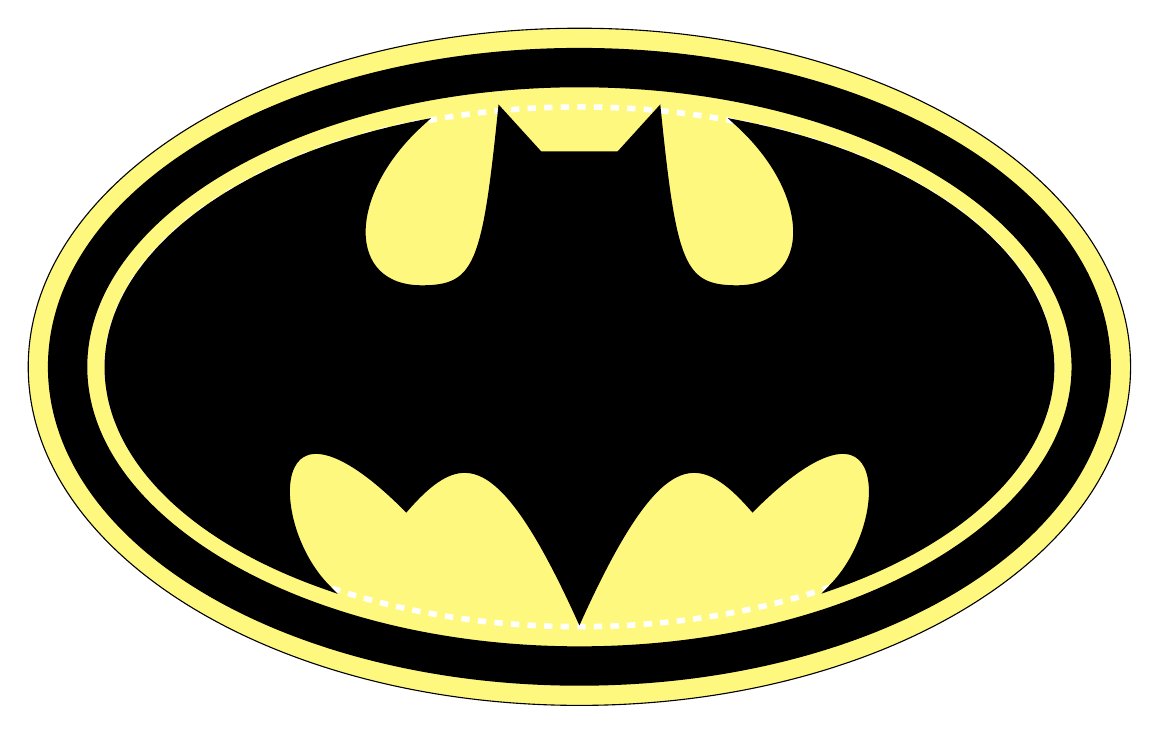
\begin{tikzpicture}

    \filldraw[fill opacity=0.5,fill=yellow] (0,0) ellipse (7.0 and 4.3);
    \draw[line width=5mm] (0,0) ellipse (6.5 and 3.8);
    \draw[line width=2pt,dashed,white] (0,0) ellipse (6.0 and 3.3);

\pgfsetlinewidth{2pt}
\pgfpathmoveto{\pgfpoint{0}{2.7cm}}
\pgfpathlineto{\pgfpoint{0.5cm}{2.7cm}}
\pgfpathlineto{\pgfpoint{1cm}{3.25cm}}
\pgfpathcurveto{\pgfpoint{1.2cm}{1.3cm}}{\pgfpoint{1.3cm}{1cm}}{\pgfpoint{2cm}{1cm}}
\pgfpathcurveto{\pgfpoint{3cm}{1cm}}{\pgfpoint{3cm}{2.2cm}}{\pgfpoint{2cm}{3.1cm}}
\pgfpatharcto{6cm}{3.3cm}{0}{0}{0}{\pgfpoint{3.2cm}{-2.8cm}}
\pgfpathcurveto{\pgfpoint{4cm}{-2cm}}{\pgfpoint{4cm}{0}}{\pgfpoint{2.2cm}{-1.8cm}}
\pgfpathcurveto{\pgfpoint{1.5cm}{-1cm}}{\pgfpoint{1cm}{-1cm}}{\pgfpoint{0cm}{-3.2cm}}
\pgftransformcm{-1}{0}{0}{1}{\pgfpointorigin} % This is the coordinate change from x to -x
\pgfpathcurveto{\pgfpoint{1cm}{-1cm}}{\pgfpoint{1.5cm}{-1cm}}{\pgfpoint{2.2cm}{-1.8cm}}
\pgfpathcurveto{\pgfpoint{4cm}{0cm}}{\pgfpoint{4cm}{-2cm}}{\pgfpoint{3.2cm}{-2.8cm}}
\pgfpatharcto{6cm}{3.3cm}{0}{0}{1}{\pgfpoint{2cm}{3.1cm}}
\pgfpathcurveto{\pgfpoint{3cm}{2.2cm}}{\pgfpoint{3cm}{1cm}}{\pgfpoint{2cm}{1cm}}
\pgfpathcurveto{\pgfpoint{1.3cm}{1cm}}{\pgfpoint{1.2cm}{1.3cm}}{\pgfpoint{1cm}{3.25cm}}
\pgfpathlineto{\pgfpoint{0.5cm}{2.7cm}}
\pgfpathclose
\pgfusepath{fill,stroke}   


\end{tikzpicture}
\end{document}